%!TeX root=MemoriaTFG.tex

%Introduction to GPS: The Global Positioning System
%OGC® Geography Markup Language (GML) — Extended schemas and encoding rules

\chapter{Conceptos principales}

En este capítulo se realiza una introducción al lector de los conceptos básicos y las 
tecnologías necesarias dentro del marco de la propuesta. Se realiza a los conceptos de sistemas de 
navegación por satélite, qué tipos principales existen, qué tipos de formatos de 
datos que encontramos y las herramientas principales a tener en cuenta para el tratamiento de datos 
geoposicionales.

\section{Sistemas de navegación por satélite} \label{}
Los \ac{GNSS} son mecanismos de detección de coordenadas geográficas formados por una constelación 
de satélites en órbita utilizados para situar elementos en la superficie terrestre. Estos sistemas permiten 
detectar las coordenadas de posición en un tiempo determinado con relativa exactitud en cualquier
punto del planeta, las 24 horas del día y en cualquier situación meteorológica \cite{Garrido-Villen01}.

Destacan entre muchos sistemas operativos en la actualidad los sistemas GALILEO, GLONASS y GPS, de 
origen Europeo, Ruso y Americano respectivamente, siendo este último el que explicaremos con más detalle 
debido a su mayor uso.

El Sistema de Posicionamiento Global, también llamado \ac{GPS} por sus siglas en inglés 
lo forma un mínimo de 24 satélites en órbita que proporcionan información de posicionamiento y tiempo 
accesible para cualquier usuario. El funcionamiento de estos sistemas se basan el cálculo de la 
distancia de un punto de la tierra a tres satélites aplicando conocimientos de "Position resection" 
\cite{Langley01}.
Esta información tiene una precisión de 100 y 156 metros para la componente horizontal y vertical, 
respectivamente al 95$\%$ de probabilidad \cite{ElRabbany01}.

Es el uso de este sistema el que permite detectar, analizar y medir la situación geográfica de un individuo, y 
esta unidad de información es el elemento mínimo de una trayectoria. En los capítulos posteriores se 
describen tanto las herramientas de manipulación de estos datos como los formatos de almacenamiento.

\subsection{GIS} \label{section:GIS}
Los Sistemas de Información Geográfica, \ac{GIS}, son aplicaciones que permiten almacenar, manipular y 
presentar la información geográfica \cite{EPA01}. Estos sistemas son usados en diferentes campos de estudio 
para el análisis y toma de decisiones. Estas herramientas permiten tratar datos relacionados con la posición de un individuo, datos de la vegetación y entorno urbanístico, permitiendo centralizar, integrar y analizar la información geográfica. Entre el gran número de aplicaciones GIS destacan ArcGIS y QGIS, 
siendo la primera software no libre publicado por la empresa Esri y la segunda software libre por la Open 
Source Geospatial Foundation.
\begin{figure}[!htb]
\begin{minipage}{0.48\textwidth}
\centering
\includegraphics[width=0.9\textwidth]{./Imagenes/ArcGIS.png}
\caption{Ejemplo de la aplicacion ArcGis}
\label{figure:ArcGis01}
\end{minipage}\hfill
\begin{minipage}{0.48\textwidth}
\centering
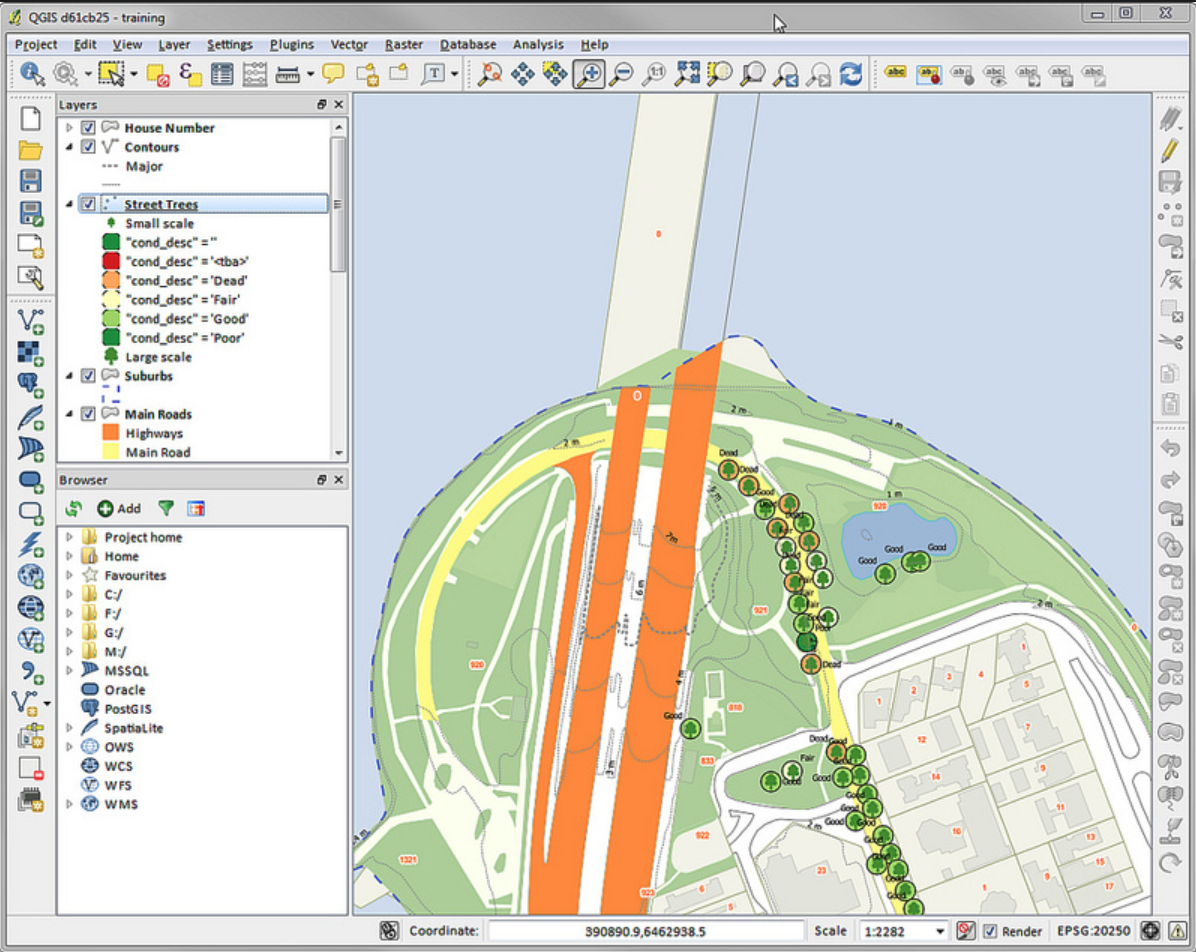
\includegraphics[width=0.9\textwidth]{./Imagenes/QGIS.png}
\caption{Ejemplo de la aplicacion QGIS}
\label{figure:QGIS01}
\end{minipage}
\end{figure}

\subsection{Fuentes de datos}
Las herramientas \ac{GIS} descritas en el apartado \ref{section:GIS} necesitan que los datos obtenidos por los 
los sistemas \ac{GPS} sigan un formato compatible. La información geoposicional es creada y manipulada y 
almacenada en múltiples formatos. Estos se dividen en dos bloques: los formatos ráster y los vectoriales. 

\subsubsection{Formato ráster}
En el formato ráster la representación de los datos se hace a partir de una malla cuadriculada. 
La geografía de un espacio queda descrita en una matriz en la que cada cuadrícula almacena la 
información como altitud o superficie. La gran ventaja que presenta respecto al formato vectorial es que 
la estructura de datos en forma de matriz es simple, no obstante consume más recursos de memoria y la 
resolución de la imagen en los límites entre los píxeles es poco definida si el número de píxeles es insuficiente.
Entre los formatos ráster más populares están Esri Grid, GeoTIFF, JPEG2000 \cite{Morales01}.

\begin{figure}[htb]
\begin{center}
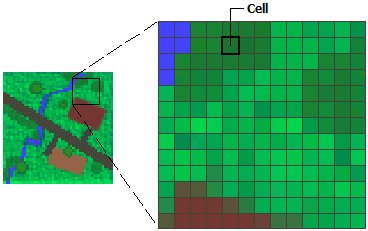
\includegraphics[width=0.6\textwidth]{./Imagenes/RasterImage.png}
\caption{Ejemplo de territorio en formato ráster. \cite{ArgGis01}}
\label{fig:PointGeneration02}
\end{center}
\end{figure}

\subsubsection{Formato vectorial}
Los formatos vectoriales se basan en la representación mediante puntos, líneas y polígonos. Presenta una
arquitectura de datos más compleja que el formato ráster, no obstante es más preciso.
De este segundo grupo destacamos los siguientes:
\begin{description}
\item [\ac{GML}] Lenguaje procedente del esquema \ac{XML} que almacena información geográfica 
\cite{OGC01}.
\item[\ac{KML}] Lenguaje basado en el esquema \ac{XML} para la representar información 
geográfica en un navegador cartográfico como Google Earth o Google Maps \cite{OGC02}.%(KML 2.1 
\item[\ac{GPX}]Formato basado en el esquema \ac{XML} para el intercambio de datos \ac{GPS}. 
En especial para la descripción de points, tracks y routes. La principal ventaja  de este formato 
es la capacidad de intercambio de datos entre diferentes  programas en diferentes entornos 
(Windows, MacOS, Linux, Palm, PocketPC). Es este el formato seleccionado como entrada de datos 
\ac{GPS} del desarrollo de este proyecto \cite{Topografix01}.
\end{description}
Es la flexibilidad de este formato y la representación independiente al tamaño del espacio geográfico 
delimitado las ventajas que determinan su uso en la continuación de la propuesta por delante del formato 
ráster.

Podemos ver en la siguiente figura un ejemplo de  una ruta de una ruta de senderismo por la Serra de 
Tramuntana (Mallorca, Illes Balears, España) en formato vectorial.
\begin{figure}[!htb]
\begin{center}
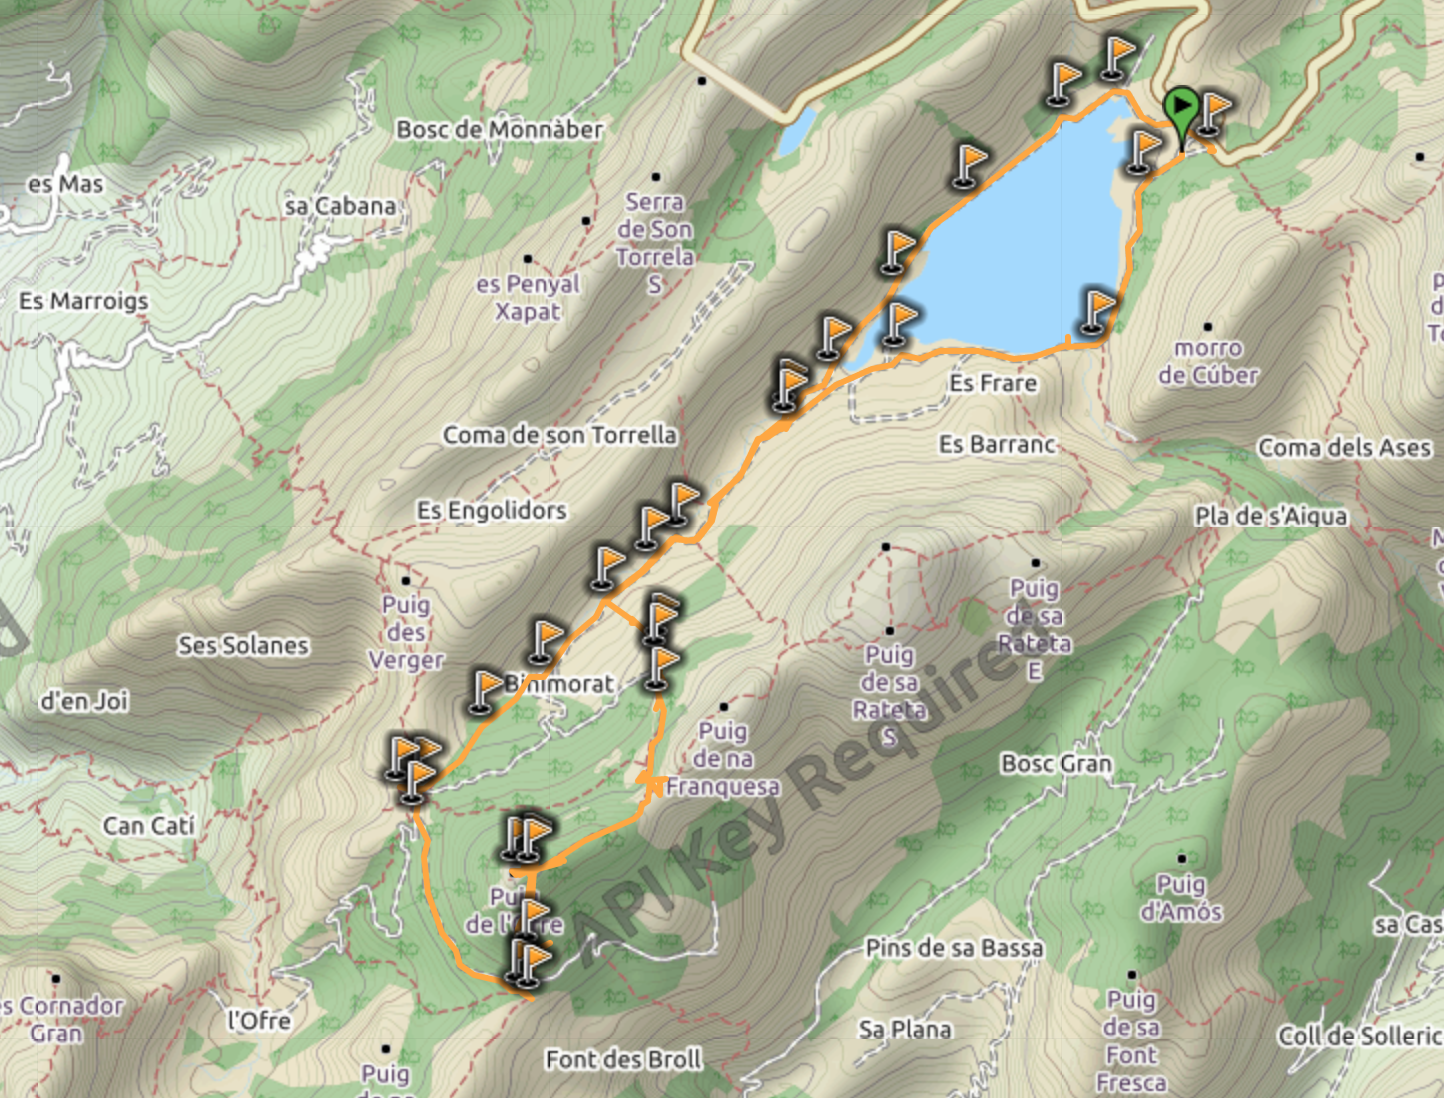
\includegraphics[width=0.5\textwidth]{./Imagenes/RutaOfre.png}
\caption{Ejemplo de Ruta del Puig de l'Ofre, Mallorca, Illes Balears, España.}
\label{figure:PointGeneration02}
\end{center}
\end{figure}
\newpage

\section{Open Street Map}
\ac{OSM} es un mapa interactivo open-source que permite visualizar información geográfica. Las gran ventaja 
de \ac{OSM} es la cantidad de herramientas aportadas por la comunidad que permiten importar, analizar, 
visualizar y editar la información. El formato de fichero \ac{GPX} es el más utilizado dentro de esta 
herramienta. La librería Osmx, que se describe posteriormente hace uso de la información de \ac{OSM} para
importar el modelo de caminos y carreteras necesario para el análisis de trayectorias. Es por lo tanto, la 
plataforma que proporciona el modelo geoespacial lógico en el que se basa la propuesta de este documento.

\section{Estructura de los ficheros \ac{GPX}}
El formato \ac{GPX} al ser basado en \ac{XML} establece sus propias etiquetas y tipos con la información 
del fichero y del espacio geográfico que describe. La etiqueta principal gpx (gpxType) es la raíz del 
fichero \ac{XML}. Presenta de forma obligatoria la versión y el creador del fichero, así como una cabecera 
de metadatos, dónde se describe la información del fichero, autor, así como restricciones de copyright 
de ser necesario. Los elementos esenciales para la descripción de la información geográfica son los 
siguientes:
\begin{description}
\item[\textit{Waypoints} (wptType)] Representación de un punto de interés. Consta de una secuencia de 
elementos 
opcionales para añadir posición, descripción y precisión, así como los atributos obligatorios de latitud/
longitud. Es la unidad mínima de detección de posición geográfica.

\item[\textit{Route} (rteType)] Lista ordenada de Waypoints.  Representan una sucesión de puntos hacia un 
destino. Contiene una secuencia de elementos descriptivos de carácter opcional. No es una representación
de un camino hecho, sino que es la unión de segmentos para llegar de un punto inicial a un punto final. 

\item[\textit{Tracks} (trkType)] Lista ordenada de puntos que escriben un camino realizado. Contiene el 
mismo tipo de secuencia de elementos descriptivos de carácter opcional. La diferencia con una \textit{Route}
es la información que representa. En este caso si que se trata de una detección de un recorrido real.
\end{description}

El formato de una trayectoria en formato \ac{GPX} parte de un \textit{track} inicial, identificado con el tag 
<trk>. El interior está formado por una sucesión de almenos un \textit{segment}, tag <trkseg>, que contienen 
a su vez la unidad mínima, un \textit{point} (<trkpt>). La información que el formato \ac{GPX} permite analizar 
en cada uno de los elementos es diversa. La latitud y la longitud de los elementos \textit{point} es información 
requerida obligatoria para la generación de un fichero \ac{GPX} válido. 
En el algoritmo \ref{algoritmo: fichero GPX} se observa un ejemplo de un fichero \ac{GPX}:

\begin{lstlisting}[caption={Ejemplo fichero GPX \cite{Gpsvisualizer01}} \label{algoritmo: fichero GPX},language=XML] 
<gpx creator="GPS Visualizer https://www.gpsvisualizer.com/" version="1.0">
  <wpt lat="45.44283" lon="-121.72904"><ele>1374</ele><name>Vista Ridge Trailhead</name><sym>Trail 
  Head</sym></wpt>
  <wpt lat="45.41000" lon="-121.71349"><ele>1777</ele><name>Wy'East Basin</name></wpt>
  <wpt lat="45.41124" lon="-121.70404"><ele>1823</ele><name>Dollar Lake</name></wpt>
  <wpt lat="45.39260" lon="-121.69937"><ele>2394</ele><name>Barrett Spur</name><sym>Summit</
 sym></wpt>
  <trk>
    <name>Barrett Spur 1</name>
    <extensions>
      <line xmlns="http://www.topografix.com/GPX/gpx_style/0/2">
        <color>9900ff</color>
      </line>
    </extensions>
    <trkseg>
      <trkpt lat="45.4431641" lon="-121.7295456"></trkpt>
      <trkpt lat="45.4428615" lon="-121.7290800"></trkpt>
      <trkpt lat="45.4425697" lon="-121.7279085"></trkpt>
      <trkpt lat="45.4102075" lon="-121.7140608"></trkpt>
      <trkpt lat="45.4099806" lon="-121.7134527"></trkpt>
    </trkseg>
    <trkseg>
      <trkpt lat="45.4099792" lon="-121.7134610"></trkpt>
      <trkpt lat="45.4091489" lon="-121.7134937"></trkpt>
      <trkpt lat="45.4086133" lon="-121.7132504"></trkpt>
      <trkpt lat="45.4080616" lon="-121.7127670"></trkpt>
      <trkpt lat="45.3928117" lon="-121.6995661"></trkpt>
    </trkseg>
    .
    .
    .
  </trk>

\end{lstlisting}